\documentclass[12pt, a4paper, oneside]{article} % Paper size, default font size and one-sided paper
%\usepackage[dcucite]{harvard}
\usepackage{tikz}
\usetikzlibrary{shapes, shadows, arrows}
\usepackage{rotating}
\usepackage{amsmath}
%\usepackage{setspace}
\usepackage{pdflscape}
%\usepackage[flushleft]{threeparttable}
%\usepackage{multirow}
\usepackage[comma, sort&compress]{natbib}% Use the natbib reference package - read up on this to edit the reference style; if you want text (e.g. Smith et al., 2012) for the in-text references (instead of numbers), remove 'numbers' 
\usepackage{graphicx}
\graphicspath{{./Figures/}} % Specifies the directory where pictures are stored
%\bibliographystyle{plainnat}
\usepackage{listings}
\bibliographystyle{agsm}
\usepackage[colorlinks = true, citecolor = blue, linkcolor = blue]{hyperref}
%\hypersetup{urlcolor=blue, colorlinks=true} % Colors hyperlinks in blue - change to black if annoying
\begin{document}
%\renewcommand[\harvardurl]{URL: \url}
\title{Carry trade and transission}
\author{Rob Hayward\footnote{University of Brighton Business School, Lewes Road, Brighton, BN2 4AT; Telephone 01273 642586.  rh49@brighton.ac.uk} and Prof. Jens H\"{o}lscher\footnote{Professor of Economics, Bournemouth Business School, Bournemouth University, jholscher@bournemouth.ac.uk, Tel: 01202 965392.}} 
\date{\today}
\maketitle
\begin{abstract}
Hyman Minsky argued that financial instability would increase through an evolution that ran from stability to precarious instability, from one characterised by \emph{hedge financing} into successively more fragile regimes of \emph{speculative financing} and \emph{Ponzi financing}.  Though this process is not directly observable, there are financial market outcomes that are more likely to be prevalent in each of these regimes.  Analysis of \emph{carry trade} returns, the attempt to take advantage of deviations from \emph{uncovered interest partiy} (UIP), is used to identify the stages of increasing financial fragility.  Return characteristics change as financial instability develops so that the process can be modeled as a Markov chain where the states are unobserved but the outcomest are conditional on  the financial regime.  The parameters of a Hiden Markov Model (HMM) can be used to aid understanding of evolution in the vlunerabilty of the financial system.  %some additional points on bubbles and conclusions can be added.  

\end{abstract}

\section{Introduction}
\subsection{The propogation of credit and liqudity shocks}
International financial conditions following the 2007-08 crisis have fuelled the growth of investments in emerging and transition economies by providing large amount of funding-currency liquidity and relatively attractive investment oppoprtunities. However, the indiction from Federal Reserve Chairmn Ben Bernanke on May 22nd and December 18th 2013, hinting that the central bank would cut back its pace of liquidity inject by gradully reducing its monthly bond purchase triggered a sharp sell-off in emerging bond and equity markets as well as their associated currencies.  This market reaction has brought attention back to relationship between US monetary policy and the flow of capital to emerging economies.  

This has drawn attention to the effect of a change in Fed policy may have on capital flows to emerging and transition markets.  For example, \citet{IMFLatam}  Uses a panel VAR method to assess the effect of US monetary policy since 1990 on capital flows to 38 emerging economies, finding evidence that Fed tapering while not necessarily leading to capital outflow, could generate \emph{new risk premium shocks}.   Similarly, \citet{NYFedtaper} assesses changes in global risk aversion on strategies that borrow low interest rates to invest in higher yields.  They find that the initial signal from the US central bank in Fed Chairman Bernanke's May 22 2013 testimony to Congress coinciced with an increase in global risk aversion which affected global asset prices. They use the approach presented by \citet{MertensSVAR} to estimate the effect of policy changes by using a two-stage least squares appraoch to identify the SVAR model of asset price changes.  By identifying the performance of exchange rates without a change in risk aversion, they find that nearly half of the depreciation of a basket of 45 carry-trade currencies with the largest one-month interest rate relative to a basket of the US dollar and other equally low rate currencies is explained by the increased risk aversion. Using a similar method they find that nearly all the decline in Emerging market equities is attributable to the increase in risk aversion.

\citet{Cerutti2014} ask three questions:  what drives global liquidity. where does the global liquidity cycle originate and how can the borrowing country manage its exposure to global liquidity? The focus is on cross-border banking flows. GLobal liquidity is affected by uncertainty and risk aversion.  This can be be captured by the VIX indx \citet{Rey2013}. US domestic conditions also affect the supply of international liquidity.  \citet{Bruno2014} suggests that domestic credit growth or the TED spread may be useful indicators. Monetary policy, as measured by short-term interest rates are also important \citet{Cerutti2014}. They have three specific findings:  an increase in the VIX index and reduction in US dealer bank leverage and a rise in the term premia reduce cross border bank lending.  There is also a small interest rate effect but this is smaller.  This suggests that global liquidity is affected by global financial conditions rather than monetary policy (though, they are of course related). 

\citet{Cerutti2014} finds that uncertainty and risk-aversion is highly correlated across countries. However, bank conditions and monetary policy actions in countries outside the US can have an influence. In a comparison of the effect of US and European domestic credit conditions and monetary policy affect lending to Asia (to remove regional influence).  Leverage conditions and TED spreads in Europe are more important for lending to Asia.  US interest rate features are the most important. They conclude that while the US drives the global liquidity cycle through its monetary policy, other financial centers (particualrly European) affect the financial cycle through the conditions of their banks. 

\href{http://www.federalreserve.gov/pubs/feds/2014/201446/201446abs.html}{Fed Paper} on flight-to-safety (FTS).  FTS episodes for 23 countries are identified from stock and equity returns.  These comprise less than 3\% of the sample.  Most of the events are country specific and are identified with an incresae in the VIX and the TED spread, falls in consumer sentiment indices and appreciations of the yen, swiss franc and US dollar. Financial, basic materials and industrial industries under-perform in FTS periods while telecoms outperform; money market instruments, corproate bonds and commodity prices (other than precious metals) face abnormal negative returns, hedge funds (particularly "event-driven" display negative FTS beta.  Liquidity deteriorates on FTS days in bond and equity markets. Economic growth and inflation decline in the year after a FTS event. 

\href{http://www.imf.org/external/pubs/cat/longres.aspx?sk=41655.0}{IMF:  Impact of Fed tapering annoncement on emerging markets}.  Using daily data on exchange rates, stock prics and emerging market bonds, exchange rates and bonds were less affected by international liquidity shocks than stock markets and were more likely to reflect domestic fundamentals (stronger macroeconomic fundamentals and policy as well as more developed financial markets. 

\citet{Ahmed2014} studies the determinants of private capital flows to emerging markets, finding that growth, interest rate differentials and global risk appetite are important.  They find that capital flows have been more sensitive to interest rate differentials since the crisis. There is also some evidnece that quantitative easing has had some effect on capital flows. 

There is evidence that the international financial cycle is increasingly global.  Rey 2013, Obstfeldt 2014 and Bruno and Shin 2014.  \href{http://www.voxeu.org/article/primer-global-liquidity}{VOX: GLobal Financial Liquidity}. For example, there is evidence the correlation of cross-broder credit growth has increased since the 1990s. Funds increasingly flow from the finacial centers to the rest of the world. As such, the G4 (term used by VOX - Claessens and Ratnovski as US, Eurozone, UK and Japan), credit and liquidity condictions affect the rest of the world. How is global liqudity measured? Global liqudity is "those credit supply factors in financial center economies that affect the provision of cross-broder credit".  Under this definition, it is specific to global funding liquidity. It is different from financial market liquidity. Therefore, financial conditions and polcy in G4 countries affect financial conditions globally. 


\subsection{Carry trade}
%Does this go somewhere else.  
One specific part of the range of international capital flows that has attracted particular attention is the \emph{carry-trade}.  This is the attempt to take advantage of the break down in \emph{uncovered interest partity} (UIP) by funding an investment in relatively high yielding transition currencies with a low interest base.  UIP is the theory that interest rate differentials between currencies shoud be matched by an equal expectation that the low rate currency will appreciate against the higher rate until expected returns from the activity are reduced to just a compensation for taking risk. The base currencies are the US dollar, the Euro, the Swiss franc and the Japanese yen.  These are the safe-haven currencies used in \citet{HabibStracca}.  The carry-trade transfers credit booms in developed economies to the rest of the world and draws developed financial institutions up against the emerging financial institutions in other countries. The carry-trade also represents a broader proxy for international portfolio flows.   

There is wide spread evidence that UIP does not hold on average but this does not mean that excess returns are possible.  It is suggested that these returns disappear with a more multifacetted assessment of risk is taken.  Most noteably, the small risk of a large loss, so-called \emph{crash risk} is either something that is to be avoided by most investors who are willing to pay to transfer this risk to other entities or is something that mis-perceived by myopic, over-confident economic agents suffereing behavioural biases.  Maybe expand this to discuss the crash risk more fully. 

%Do the next two paragraphs set up the dicotomy between the domestic factors and the international (flight-to-quality) factors?  THere are a range of facts:  EM debt rose from 650bn in 2001 to 6.9tn in 2013 according to BIS data.  

\subsection{CEE}
Economies in transition have faced repeated struggles with financial instability.  The pressure to open economies to international finance has exacerbated this risk as it has added a huge stock of international financial capital to the potential flow that can enter during the country during the optimistic expansionary stage with more significant and adverse consequences when the it retreats.

When economies are in trasition, economic norms and institutions are changing and it becomes easy to downplay the likelihood that previous economic shocks will be repeated.  The idea that conditions are new gains weight.  Financial system tend to be less developed and therefore there is scope for finance to increase in absolute terms as well as relative to overall level of economic activity.  This process can attract financial entities from more developed economies. \citet{ONBcarry} and \citet{EBRD} surbvey the expansion of Euro area banks into the Central and Eastern European trasition economies; \citet{Gabor} discusses the political economy of this \emph{financialization} where the financial system expands to new sections of the economy.  

Money flows in and it can retreat just as swiftly.  The evolution of financial risk is familiar. \citet{DornbuschSS}, \citet{CalvoSS} and \citet{KrugmanSS} have been associated with the term \emph{sudden stop} to emphasise the importane of the inflow that takes place before the currency crisis in understanding the disruptive effects of the reversal.   

%other references 
 %Abiad, A., 2003. Early-Warning Systems: A Survey and and a Regime-Switching Approach. IMF Working Paper No.03/32. International Monetary Fund.
 %Aziz, J., Caramazza, F., Salgado, R., 2000. Currency Crises: In Search of Common Elements. IMF Working Paper No.00/67. International Monetary Fund
 %Calvo, G., 2000. Balance-of-Payments Crises in Emerging Markets: Large Capital Inflows and Sovereign Governments, in: Krugman, P. (Ed.), Currency Crises, University of Chicago Press, Chicago, Illinois,
 \href{http://mpra.ub.uni-muenchen.de/383/}{http://mpra.ub.uni-muenchen.de/383/}

As such, there is increased skepticism about the benefit of the free flow of international capital since the dispuptive currency crises spilt from Mexico through Asia, Russia and other parts of the world in the 1990s.  In addition, the story of \emph{global imbalances} and the phenomenon of developing China lending to the US flies in face of the theory that suggests that rich developed countries will aid the progress of the less developed by providing the funding for deepening of capital.  

\subsection{The instability cycle}
The aim is to get some view of the factors that drive movement from one regime to another.  What are the factors that surround a move from caution to the building of risk and what are the factors that are associated with the movement from risk-building to collapse?  Minsky provides a very powerful description of the financial instability cycle.   There have been a number of attempts to identify levels of finacial risk.  This has clearly become even more of an issue since the financial crisis. Referenes (BIS etc measurements????).  For example, \citet{IFCMeasure}.  The IMF have developed a range of \emph{Financial Soundness Indications} (IMF 2006).     Also - Hawkins and Klau (2000), Nelson and Perli (2005) and Gray et al (2007).  There are six main strands:  the real sector, including fiscal position and inflation; the corporate sector, specifically the level of debt and overseas exposure; the ability of the household sector to weather downturns; the external sector, including the foreign exchange position and the capital account; the financial sector; finacial markets. 

%A number of studies applied the early warning indicator methods initially developed in the literature for currency and balance of payments crises to banking crises. Earlier work includes, among others, Calvo et al (1993), Eichengreen et al (1996), Turner and Goldstein (1996) Frankel and Rose (1996). Demirgüç-Kunt and Detragiache (1997) use a multivariate Logit approach to identify determinants of banking crises in a large panel of developing and industrialised countries: slow GDP growth and high inflation, vulnerability to sudden capital outflows, low liquidity in the banking sector, a high share of credit to the private sector, past credit growth, explicit deposit insurance and weak institutions. Kaminsky and Reinhardt (1999) identify early warning indicators of twin (banking and balance of payments) crises, such as credit and equity prices, by looking at the ability of such variables to predict crises 12 or 24 months ahead, while minimising the noise3  to signal ratio. Borio and Lowe (2002) and Borio and Drehmann (2009) build on the techniques developed by Kaminsky and Reinhardt (1999). Like the latter, they define threshold values for the indicators, but unlike them, they look at cumulative processes rather than just growth rates over one year, they use ex ante information (ie information which was available to the policymaker prior to the crisis) and, for the first time, they consider combinations of indicators and look at multiple time horizons. BIS Goodhart 2006%


How can the evolution of financial conditions be assessed?  While measuring debt-to-equity ratios and the scale of bank lending may provide some indication about the regime that is in place, this is imprecise and it is clear that financial services business evolve in ways that make loan counting  inadequate.The recent financial crisis showed that innovations like \emph{Collateralised Debt Obligations (CDO)} can allow an increase in debt that does not directly in bank lending. There are two ways to try to identify the regimes: use external indicators such as the VIX index or other indications of domestic economic or political uncertaintly; use the internatl structure of the data to identify the periods through which the financial system  is evolving.  

\subsection{Minsky's Financial Instatility Hypothesis}
Minsky's \emph{Financial Instability Hypothesis} (FIH) presents a model of endogenous financial crisis where a period of economic calm creates the conditions for more adventorous and risky financial behaviour that increases the fragility of the system.  Minsky identified three phases of financing:  hedge, speculative and Ponzie.  

In the first of these the system is stable as lending is not excessive, borrowers are cautious and revenues are generally sufficient to ensure that repayments of principal and interest can be made from current income.  This period may be framed by memories of past financial crisis and the economic hardships that are associated with it.  Violent economic shocks are among the range of possible outcomes that are envisaged by creditors and debtors, encouraging them to be cautious and risk-averse. 

However, in the absense of economic shocks these memories of hardship fade further into the background and all parts of the economic and financial system become more prepared to take risks.  Lending becomes more speculative; decision-making gives less weight to the possibility of extereme outcomes and more weight to the immediate experience of economic calm.  The increase in lending tends to improve immediate economic conditions:  business investment and consumer spending increase if lending is broad-based; asset prices will rise where lending is directed towards financial investment.  The increase in economic activity that comes from this expansion in credit will feedback to improve immediate economic conditions, exacerbating the sense of well-being and undermining the arguments of those preaching more cautious behaviour.  

\citet{Bernanke1999chapter}, \citet{BernankeGertler} and \citet{Azaraidis} present models where there is a non-linear relationship between  the provision of credit and the level of economic activity. \citet{BernankeGertlerAgency} provide a model where balance sheet dynamics affect the business cycle through a reduction in the agency cost of business investments and \citet{Balke} has a non-linear model of credit shocks.  \citet{Avdjiev2014} use a three regime TVAR model to identify the non-linearities in credit market shocks.  They find that credit shocks have the creates impact when output growth is above its long-term trend. 

While credit becomes more plentiful, household and business managers become more optimistic.  There is evidence that decision-making tends to favour occurances that can be more easily envisaged or those that are more recently arrived (see for example, \citet{KTAvailability} and \citet{Schwartzavailability} for some evidence on the \emph{availability heuristic}.   % more required or footnote? 

In this way, the repayment of loans becomes increasingly dependent on the continuation of above-norman economic conditions or the appreciation of asset prices.  If this process is allowed to continue a speculative frenzie can take hold.  Economic agents are dragged into the euphoria as households compete with the conspicuous consumption of their neighbours, businesses make investments to increase capacity to meet booming demand and endovour to increase market share, while property and financial market speculators redouble their bets.  \citet{BrunnermeierLiquidity} show how the link between the availability of credit for investors and the level of liquidity in financial markets can create \emph{liquidity spirals}.   They note, in particular, that the capital of speculators can drive market iquidity, risk premia and asset prices.  The ability to be able to borrow against collateral is particularly important here.  As asset prices increase, the ability to borrow against their value increases the amount of trading credit that is available.  

The conditions are now in place for the bubble to burst in a violent reversal.  \citet{FisherBD, FisherDD} explained the way that \emph{debt-deflation} could create a ricochet between the financial and real sectors of the economy with a decline in the availablity of credit exacerbating the financial strain on households and business, helping to reduce household and business spending thereby raising the level of bad loans and the level of caution at financial instiutions. In financial markets, credit and liquidity disappear and decline in asset values affect the ability of insitutions to raise funds.  Firesales in illiquid markets exaggerates the fall in prices. \citet{ReinhartRogoff} show how credit booms help to explain the breadth and depth of post-boom recessions.  The catalist for the collapse is difficult to pin down as the build up to the excess is fragile.  However, the economic consequences are profound.  


\section{The evolution of financial riskl}
As the financial system evolves from a position of caution into one where risk is being built and finanlly into a precarious position where collapse takes place, the nature of the returns to the carry-trade will change. Durhing the period caution there is a small excess return, as risk is built the returns will tend to increase to reflect the fact that the building of carry positions will tend to add a capital appreciation in the exchange rate to the interest rate pick up. During the crash, there are losses and extreme risk.   The probability a particular tupe of return depends on the type of return that was seen in the previous regime.   For example, probability that the carry-trade will provide a good return with minmum risk will be greatest when that was the previous regime:  if this speculative activity is profitable and others are attracted to the activity, the possibility of a crash is limited.  However, there is some modest probability of a crash and some probability that there could be a return to caution. .  In other words, there is a sequence from one financial state to another and there are probability that can be applied to being in each of these states and to making the transiton from one state to another.

%\begin{centering}
%\begin{tabular}{l l l l}
% & Crisis & Specultion & Caution \\
% Crisis & $P(Cr|Cr)$ & $P(Cr|Sp)$ & $P(Cr|Ca)$\\
% Speculation & $P(Sp|Cr)$ & $P(Sp|Sp)$ & $P(Sp|Ca)$\\
% Caution & $P(Ca|Cr)$ & $P(Ca|Sp)$ & $P(Ca|Ca)$ \\
% \end{tabular}
%\end{centering}

The regimes of financial instability are not observed.  However, the returns to the carry trade will change as the regime changes:  in the calm phase there may be a very small return that reflects the failure of UIP to hold on average; in the specualtive phase, carry-trade positions are built more agressively and this encourages an increase in returns as the interest rate carry itself is combined with the capital appreciation that come from sales of funding currency and the purchase of investment currency.  It also reduces risk as evident in the standard deviation of these returns. The crisis is the period of crash and reversal.  The HMM aims to find the probability of a particular pattern given a particular state. The three latent states are the periods of caution, build and crash.   

The returns depend on the underlying financial regime.  For example, if there are steady returns being made from the carry-trade, the probability that these returns continue in the next period or that there is a crash or a return to caution will depend on the underling financial regime:  if the financial regime is speculative, the probability of retaining good returns or moving to a crash will be relatively high and the probabiluty of returning to caution will be relatively low; if the the financial system is in a position of calm, there is a greater probability that there can be a return to caution and a smaller chance of a crash.  The transition matrix is differenet for different regimes. 

There is also an %\emph{HMM emission matrix}
which gives the probabilities of each return type in each of the financial regimes. For example, in the spculative phase, the probability of speculative returns is high, there is some probability of crash and some probabilty of caution. 

Give this information, it is possible to construct a sample of carry-returns from the initial probabilities, the transition matrix and the emission matrix.  Alternatively, it is possible to work backwards from the carry returns using the  transiton matrix and the emission matrix to find the most likely sequence of financial states by applying the \emph{viterbi} algorithm (see Chapter10.R for full details of how this works).  

\begin{landscape}
\begin{figure}
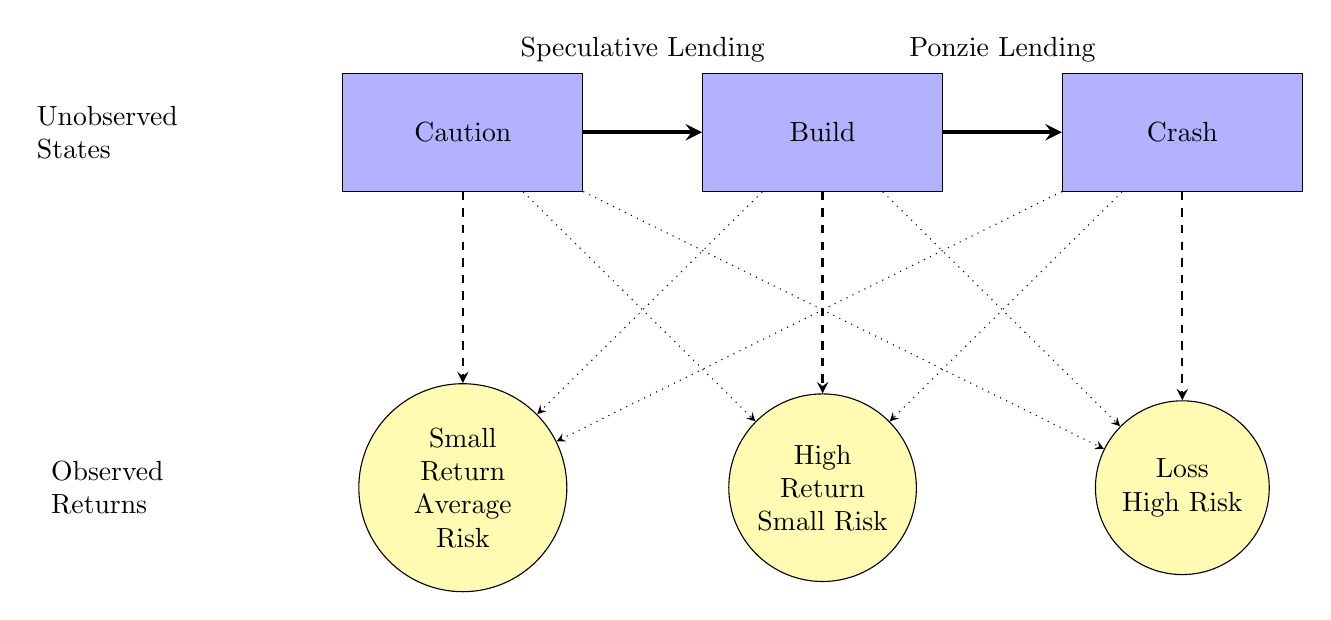
\begin{tikzpicture}
\tikzstyle{decision} = [circle, draw, fill = yellow!30, minimum height = 8mm, 
  text width = 5em, text centered];
\tikzstyle{line} = [draw, -stealth, thick]
\tikzstyle{line2} = [draw, -stealth, ultra thick]
\tikzstyle{line3} = [draw, -stealth, dashed, thick]
\tikzstyle{line4} = [draw, -stealth, dotted]
\tikzstyle{elli} = [draw, ellipse, fill = red!50, minimum height = 8mm, 
  text width = 5em, text centered]
\tikzstyle{block} = [draw, rectangle, fill = blue!30, text width = 8em, 
	text centered, minimum height = 15mm, node distance = 8em]
\node [block](Build){Build};
\node [block, left of  = Build, xshift = -5em] (Caution){Caution}; 
\node [block, right  of = Build, xshift =5em] (Crash){Crash};
\node [decision, below of = Build, yshift = -10em, align = center]
(Build2) {High Return \\ Small Risk}; 
\node [decision, below of = Crash, yshift = -10em](Crash2) {Loss \\ High Risk};
\node [decision, below of = Caution, yshift = -10em, align = center](Caution2) 
{Small \\ Return \\ Average \\ Risk};
%arrows 
\path [line3] (Caution) -- (Caution2);
\path [line3] (Build) -- (Build2);
\path [line3] (Crash) -- (Crash2);
\path [line2] (Build) -- node [yshift = 3em] {Ponzie Lending} (Crash);
\path [line2] (Caution) -- node [yshift = 3em]  {Speculative Lending} (Build);
\path [line4] (Caution) -- (Build2);
\path [line4] (Caution) -- (Crash2);
\path [line4] (Build) -- (Crash2);
\path [line4] (Build) -- (Caution2);
\path [line4] (Crash) -- (Caution2);
\path [line4] (Crash) -- (Build2);
\node [align = left, left of = Caution, xshift = -10em] {Unobserved \\ States};
\node [align = left, left of = Caution2, xshift = -10em] {Observed \\ Returns};
%\path [line] (decision1) -| node [yshift = 0.5em, 
% 	xshift = 8em] {YES} (process 1);
%\path [line3] (Crash) -- (Caution); 
% 	xshift = -8em] {NO} (process 2);
\end{tikzpicture}
\caption{Hidden Markov Model (HMM)}
\label{fig:HMM}
\end{figure}
\end{landscape}



\subsection{The Hidden Markov Model (HMM)}
The mathematical model goes here after the explanation above.  


From Maatin's London R:  reference the package.  In a \emph{mixture model}, each observation is assumed to be drawn from a number of distinct sub populations.  These can be called \emph{component distributions}.  The distribution from which the component is drawn is not immediately observable and is therefore represented as a \emph{latent state}.  Here the state is the unknown financial regime.  

A mixture distribution is defined as 
\begin{equation}
p(Y_1 = y) = \sum_{i - 1}^N p(Y_t = y|S_t = i)P(S_t = i)
\end{equation}
where,
\begin{itemize}
\item $S_t \in {1, \dots, N}$ denotes the latent state or class of observation t
\item $P(S_t = i)$ denots the probability of the latent state t equals i 
\item $p(Y_t = y|S_t = i)$ denotes the density of observation of $Y_t$ conditional on latent state being $S_t = i$.
\end{itemize}

In the \emph{dependent mixture model} states are assumed to be statistically dependent.  This is consistent with the Minsky theory that the period of calm creates the conditions for the crash. The process underlying the state transitions is a \emph{homogenous first order Markov process}  (look this up for additional definition).  This process is completely defined by the initial state probabilities.  

\begin{equation*}
P(S_1 = 1), \dots P(S_1 = N)
\end{equation*}
and the state transition matrix, 

\begin{equation*}
\begin{pmatrix}
P(S_t = 1|S_{t-1}=1) & P(S_t = 2|S_{t-1}=1) & \dots & P(S_t = N|S_{t-1}=1)\\
P(S_t = 1|S_{t-1}=2) & P(S_t = 2|S_{t-1}=2) & \dots & P(S_t = N|S_{t-1}=2)\\
\vdots & \vdots & \ddots & \vdots \\
P(S_t = 1|S_{t-1}=N) & P(S_t = 2|S_{t-1}=N) & \dots & P(S_t = N|S_{t-1}=N)
\end{pmatrix}
\end{equation*}

The models are estimated using the Expectation-Maximisation (EM) or numerical optimisation (when parmeters are constrained).  The dependent mixture model is made up of three sub models:  
\begin{enumerate}
\item The prior model: $P(S_1|x, \theta_{prior})$
\item The transition model: $P(S_t|x, S_{t-1}, \theta_{trans})$
\item The response model: $P(Y_t| S_t, x, \theta_{resp})$
\end{enumerate}
 
In this case, 

The regimes are
\begin{itemize}
\item Hedge: cautious and risk averse
\item Speculative: More willing to take increased risk. 
\item Ponzi:  Risk-loving and explosive
\end{itemize}


The raw model just assume that there are three states with random allocation of the starting values.  However, the initial estimates of the regime parameters can come from the estimates made in the doctorate using the crash and caution identification from the VIX; the initial estimates of the priobabilities of each state can come from the percentage of each state in the final version of the model that is run without initial estimates.  

I think that $\theta_1$ on page 4 of the depmixS4 vignette is the parameter that nees to be set. 

it woould be useful to see which of the two models works best: the standard idea of high risk and crash or the Minsky model.  

In the case of the PLNUSD (actually PLNEUR) it seems from the derived transition matrix and the information criteria as if the two-regime model has a better fit than the three regime model. 

At the top of page 10 of the vignette, there is an example of how the transition matrix may be augmented by a model.  I do not understand this fuilly, but it may be possible to link the transition to the VIX index.  Obviously, there is some risk of circularity here. Anyway, it may be useful to compare the difference. 

Second page of the model.  There will be overlaps that need to be cut out and re-written. 

\subsection{Formal model}
\href{http://en.wikipedia.org/wiki/Hidden_Markov_model}{Hidden Markov Models}.  
$f(y_{it}|z_t)$ is assumed to have a multivariate normal density function. This distribution is characterised by $\theta_k = (\mu_k, \sigma_k^2)$.  Excluding the states $w$, there are the initial state probabilities to be determined, the 2 transition probabilities and the conditional mean and conditional variance to be estimated.  Thsi is done by Maximum likelihood using the log-likelihood function $l(\varphi, y) = \sum_{i=1}^n log f(y_i; \varphi)$. This is a problem that can be solved with the \emph{Expectation-Maximization (EM) algorithm} \citet{dempster1977maximum}. The E step computes the joint conditional distribution of the latent variables given the data and the current provisional estimates of the model parameters. The M step ML methods are used to update the parameters using the estimated densities of the latent variables as weights. For hidden Markov models, as special variant of the EM algorithm is proposed (called \emph{the forward-backward} or \emph{Baum-Welch} alogorithm (Baum et al 1970).   

Notes from the \href{http://www.comp.leeds.ac.uk/roger/HiddenMarkovModels/html_dev/main.html}{Leeds notes}.  The aim is to find patterns in time. This uses the examle of seaweed and traffic lights.  For the traffic lights, there is a state machine where the different states follow each other. Each state is dependent only on the previous state. This is a deterministic system. The weather is not deterministic.  There may be three states:  wet, cloudy and sunny. The Makov assumption says that the state depends only on the previous state. This is a simplification that makes the problem easier to solve.  Some information may be lost with the simplifcation. The Markov process moves from state to state, depending only on the previous n states.  This is called an \emph{order n model}, where n is the number of states affecting the choice of the next state. With the weather example there are 9 possible transformations $(M^2)$.  The probability of each transition is assigned  a probability called \emph{state transition probability}.  These are collected into a \emph{state transition matrix}. The probabilities do not vary with time.  This is a (unrealistic) assumption. However, it is an assumption that can be relaxed (see below).  To start the system, there is a \emph{vector of initial probabilities}.  This is the $\pi$ vector.  These are set randomly in the current case and this random starting point can be changed so that outcomes can be compared to asssess the importance of the starting point for the results. Presumably, the starting points could also be set if there were a strong opinion on the regime that begins the time period. For example, the data begin in 1990.  Is this a time  of calm, build or crash? 

The first order Markov process has three elements: 
\begin{enumerate}
\item states
\item $\pi$ vector
\item state tansmition matrix
\end{enumerate}
 Sometimes the Markov model is not sufficient to fully describe the process.  In the weather example, the weather may not be observable but seaweed is evident.  There is a probabilistic relationship between the returns that are evident and the underlying state of the financial system.  More realistic is the identification of hidden states of the mouth through the sounds that can be identified.  The observables are related to the hidden states. It is assumed that the hidden states (the weather) are modelled by a simple first order Markov process.  The connections between the hidden states and the observable states represent the probability of generating a particular observed state given that the Markov process is in a particular state.  This is the \emph{confusion matrix} which gives the probabilites of observable states given a particular hidden state. 
 
In our case it is assumed that the hidden states representing the evolution of financial conditions according to Minsky's Financial Instability Hypothesis evolve in a way that can be modeled by simple, first-order Markov process. 
 
The Hidden Markov Model (HMM) is a tripple $(\pi, A, B)$ where, 
\begin{enumerate}
\item $\pi$ Vector of initial state probabilities
\item $A = (a_{ij})$ the state transition matrix $Pr(x_{it}|x_{jt-1})$
\item $B = (b_{ij})$ the confusion matrix $Pr(y_i|x_j)$
\end{enumerate}


\subsection{Investgations using HMM}
THere are a number of problems that can be solved.  This section may help explain the algo that is used. Otherwise, it may be discarded.  The essential steps are:  firstly, identif the probability of the observed sequence given the chosen HMM; take that sequence and fit the best possible HMM.  There should, I think, be an iteration between the two. 

Once a system can be described as HMM, three problems can be solved. 
\begin{enumerate}
\item finding the probability of an observed sequence given a HMM (evaluation)
\item finding the sequence of hidden states that most probably generated the obsered sequence (decoding)
\item generating a HMM given a sequencde of observed observations (learning)
\end{enumerate}

\subsubsection{Evaluation}
There are a number of HMM with sets of $(\pi, A, B)$ tripples, which HMM geneated the given sequence?  For example, there may be 'summer model' and a 'winter model' and it may then be possible to determine the season from the seaweed sequence. The \emph{Forward algorithm} is used to calculate the probability of an observation sequence given a particular HMM and hence the most probable HMM.  In speech recognition, the HMM represent different words and the most likey HMM determines the word. 

It may be that there are different models for fixed and floating exchange rates. 
\subsubsection{Decoding}
It is most usual to find the hidden states that generated the observed sequence.  Finding the hidden states is important because they are not directly observable.  A blind hermit may feel the seaweed but cannot see the weather. The \emph{Viterbi algorithm}.  This could also be used to determine the syntactic class of words (noune, verb etc) from the words themselves.  

What is the probability of the observed sequence given the HMM? This can evaluate risk - crash? 

\subsubsection{Learning}
This is the most difficult task.  Take a set of observations and fit the most probable HMM . The \emph{Forward-backward algorithm} is used when the A and B matrices are not directly (empirically) measurable.  

\subsubsection{Forward Algorithm}
With three states, three observations and the parameters of the model known, the aim is to find the most likely hidden sequence.  It would be possible to find each possible sequence and sum the probabilities.  





\subsection{The algo}
The \emph{Viterbi algrithm} will create a matrix v that will contain the probability of each regime, given the type of return that is evident. This is computed from the product of the transition matrix, which gives the probability of transfering to the currnt regime from the previous regime, and the maximum value of V in row i-1.  For each state, there will be a probability which is the product of the probability of seeing the regime given the returns and the most likely state in the previous period and the probability of the state given the return \begin{verbatim}v[i,l] <-  statelprobnucleotidei * max(v[(i-1),] * transitionmatrix[,l])\end{verbatim} which is line 45 of viterbi.R

Expectations-Maximisation (EM) algorithm. 


\subsection{Use of the model}
Peso
Some history, 
Some examples from genetriics and speech....

Economics and finance
Hamilton

The second paper (on rating agencies - incuded in the "other" folder.  Uses the mixture model against the alternative of a pure Markov chain. In the pure Markov chain, the future depends only on the present.  However, with the mixture model, the future depends on the past.  This means that it is impant to know which of the latent sub-groups the firm is in as this will tell you more about the probability of default.  This knowledge will be based on the whole sample of ratings. There are A and Q processs.  What determines whether the rating evolves according to A or Q?  It appears to be partly the result of the industry.  The wholesale and retail trades are the most dynamic. There is clearly a hetrogeneity that is ignored by the standard Markov model of rating migration. 

As such, it may be possible to make a comparison of developed and less developed finncial systems or fixed and floating systems.  How do they differ?  What does this tell us about how vulnerble the systems are?  


Agn Timmerman (2011)
Looking at how abrupt changes in regime can lead to changes in the way that the system works.  The different regimes can be associated with different underlying distribution of returns.  This can allow the understanding of the non-liner and non--normal distribution within  normal or linear framework.  At the extreme, the regime switch model can incorporate a \emph{jump model} with one change, and can also be associated with time-varying parameter models that have a large number of regimes.

The broad framework for the method is to model a discrete state $s_t \in \{0,1,\dots k \}$
\begin{equation}
y_t = \mu_{s_t} + \phi_{s_t} y_{t-1} + \sigma_{s_t} \varepsilon_t, \quad \varepsilon_t \sim iid(0,1) 
\end{equation}

The process governing the underlying regime must also be defined. 

\begin{equation}
Pr(s_t = 0| s_{t-1} = 0) = p_{00} \quad \text{and} \quad Pr(s_t = 1| s_{t-1} = 1) = p_{11}
\end{equation}

More generally, the transition could be time-varying and could be dependent on the time spent in the regime.  See Durland and McCurdy (1994) for example of the probbilities  in the transition matrix being related to time. The longer the systemm has remained in the build phase, the greater the risk of crash.  Remember that the crash phase is a period when there is risk of a sharp reversal.  

See Diebold, Lee and Weinbch (1994) for examples where the transition probabilities depend on some other state variables.  For example, the interest rate spread.   Could the VIX index or other factors be used?  Vix index would indicate heightened international tension as one element that affects the probability of transforming from one state to the next.  An elevated VIX is an indication of the heightened international risk premium.  This may increase the probability that the regime switches from carry build to crash.  This is a theme that could be related to the bubble bursting so any information that improves the ability to identify bubbles bursting would be beneficial.  


  There are two states of the world:  crisis and moderation.  If the system is in a crisis, it stays there with probability p; it switches to moderation with probability $1-p$.  If in moderation, the system stays there with a probability q and switches to crisis with probability $1-q$.  If the probabilities change over time, there is no longer a \emph{homogenous Markov Chain}. Ghysels has a seasonal dummy for the probabilities that represent the months or quarters.  

Can the probabilities change over time?  This may be the result of changes in the resilience of the financial system. 
\href{http://members.home.nl/jeroenvermunt/dias2010.pdf}{Mixture Hidden Markov Models} Hidden models help to calafify the regime under which securities trade. Model takes into account the unobserved hetrogeneity across time. This could could be extended to space (for different countries).  Is it possible to estimate a panel? 

Can the systemm be used to compare to fixed and floating exchange rates. 

The use of the regime-switch allows the transition from one regime to another to be the result of something that is more than just a deterministic process. There are a number of ways that this model could be expanded.  Dueker has a model where the degrees of freedom from a Student-t distribution change with the regime.  



\section{Analysis of Results}
\subsection{Data}
The data are a sample of CEE carry-trades that have been compiled from raw exchange rate and interest rate data for the period from January 2000 to December 2013.  They show a range of possible carry-trades that could have been conducted. 

The data are calculated as follows

\begin{equation}\label{eqref:carryprofit}
P1MEURHUF_t = \frac{(1 + HUF1M_t)^{\frac{1}{12}} \times EURHUF_t }{(1 + EUR1M_t)^{\frac{1}{12}} \times EURHUF_{t+1M}}
\end{equation}

where $HUF1M_t$ is the 1 month Hungarian Forint deposit rate at time t, $EUR1M_t$ is the 1-month euro denominated deposit rate at time t, $EURHUF_t$ is the exchange rate in terms of  Hungarian Forint required for one euro at time t and  $EURHUF_{t+1M}$ is the spot rate in 1 month's time.  This is fundamentally the same as \citep{BrunnermeierCarry}.

where the forward rate is calculated as

\begin{equation}\label{eqref:forward}
EURHUF_t^{f1m} = \frac{(1 + HUF1M_t)^{\frac{1}{12}} \times EURHUF_t }{(1 + EUR1M_t)^{\frac{1}{12}}}
\end{equation}

where  $EURHUF_t^{f1m}$ is the 1 month forward rate for euro in terms of Hungarian Forint at time t, $HUF1M_t$ is 1 month Hungarian Forint deposit rate, $EUR1M_t$ is the 1 month Euro deposit rate and $EURHUF_t$ is the current rate of Euro in terms of Hungarian currency.  The code for the calculation is in the function \lstinline{forp} in the package \lstinline{prepareR}. This will create a sample of carry-trade profits from an array of CEE investment currencies relative to standrd funding currencies.   The ISK, TRY and NOK are used as reference.  One month and 3 month carries are created.  It would be possible to have shorter time periods for the carry-trade.   This would require the addition of the appropriate times series for LIBOR or deposit rates.  

\subsection{Results}
Running the Raw.R file, lines 22 to 24
\begin{lstlisting}
mod <- depmix(PPLNUSD ~ 1, nstates = 3, data = da)
 set.seed(3)
fm2 <- fit(mod, verbose = FALSE)
depmixS4::summary(fm2)
\end{lstlisting}

gives the results
 
 
The parameters of the 2 regime model are given in Table \ref{tabref:2StateProb}.  They show....


\begin{landscape}
% latex table generated in R 3.0.2 by xtable 1.7-1 package
% Mon Jun 30 10:17:10 2014
\begin{table}[ht]
\centering
\begin{tabular}{rrrrrrrrrrrr}
  \hline
 & HUF & PLN & CZK & RON & RUB & TRY & BGN & NOK & ISK & UAH & HRK \\ 
  \hline
  EUR (mean) & 1.0165 & 1.0173 & 1.0129 & 1.0150 & 1.0098 & 1.0151 & 1.0075 & 1.0092 & 1.0091 & 1.0094 & 1.0091 \\ 
  Calm (sd) & 0.0519 & 0.0486 & 0.0542 & 0.0433 & 0.0310 & 0.0460 & 0.0381 & 0.0693 & 0.0532 & 0.0295 & 0.0251 \\ 
  EUR (mean) & 0.9905 & 0.9862 & 0.9963 & 0.9969 & 0.9962 & 0.9969 & 1.0053 & 1.0008 & 0.9427 & 0.9673 & 1.0082 \\ 
  Crash (sd) & 0.1085 & 0.1026 & 0.0886 & 0.0878 & 0.0779 & 0.1028 & 0.0826 & 0.0303 & 0.1871 & 0.1116 & 0.0737 \\ 
  \hline
  USD (mean) & 1.0165 & 1.0173 & 1.0129 & 1.0150 & 1.0098 & 1.0151 & 1.0075 & 1.0092 & 1.0091 & 1.0094 & 1.0091 \\ 
  Calm (sd) & 0.0519 & 0.0486 & 0.0542 & 0.0433 & 0.0310 & 0.0460 & 0.0381 & 0.0693 & 0.0532 & 0.0295 & 0.0251 \\ 
  USD (mean) & 0.9905 & 0.9862 & 0.9963 & 0.9969 & 0.9962 & 0.9969 & 1.0053 & 1.0008 & 0.9427 & 0.9673 & 1.0082 \\ 
  Crash (sd) & 0.1085 & 0.1026 & 0.0886 & 0.0878 & 0.0779 & 0.1028 & 0.0826 & 0.0303 & 0.1871 & 0.1116 & 0.0737 \\ 
  \hline
  CHF (mean)& 1.0165 & 1.0173 & 1.0129 & 1.0150 & 1.0098 & 1.0151 & 1.0075 & 1.0092 & 1.0091 & 1.0094 & 1.0091 \\ 
  Calm (sd)& 0.0519 & 0.0486 & 0.0542 & 0.0433 & 0.0310 & 0.0460 & 0.0381 & 0.0693 & 0.0532 & 0.0295 & 0.0251 \\ 
  CHF (mean) & 0.9905 & 0.9862 & 0.9963 & 0.9969 & 0.9962 & 0.9969 & 1.0053 & 1.0008 & 0.9427 & 0.9673 & 1.0082 \\ 
  Crash (sd) & 0.1085 & 0.1026 & 0.0886 & 0.0878 & 0.0779 & 0.1028 & 0.0826 & 0.0303 & 0.1871 & 0.1116 & 0.0737 \\ 
  \hline
  JPY (mean) & 1.0165 & 1.0173 & 1.0129 & 1.0150 & 1.0098 & 1.0151 & 1.0075 & 1.0092 & 1.0091 & 1.0094 & 1.0091 \\ 
  Calm (sd) & 0.0519 & 0.0486 & 0.0542 & 0.0433 & 0.0310 & 0.0460 & 0.0381 & 0.0693 & 0.0532 & 0.0295 & 0.0251 \\ 
  JPY (mean) & 0.9905 & 0.9862 & 0.9963 & 0.9969 & 0.9962 & 0.9969 & 1.0053 & 1.0008 & 0.9427 & 0.9673 & 1.0082 \\ 
  Crash (sd) & 0.1085 & 0.1026 & 0.0886 & 0.0878 & 0.0779 & 0.1028 & 0.0826 & 0.0303 & 0.1871 & 0.1116 & 0.0737 \\ 
   \hline
\end{tabular}
\caption{Mean and Standard Deviation of 2 Regime Model}
\label{tabref:2StateProb}
\end{table}
\end{landscape}

\begin{landscape}
% latex table generated in R 3.0.2 by xtable 1.7-1 package
% Wed Jul 02 10:58:12 2014
\begin{table}[ht]
\centering
\begin{tabular}{rrrrrrrrrrrr}
  \hline
 & HUF & PLN & CZK & RON & RUB & TRY & BGN & NOK & ISK & UAH & HRK \\ 
  \hline
Cautious (mean) & 0.9952 & 1.0004 & 0.9954 & 1.0007 & 0.9957 & 1.0005 & 1.0094 & 1.0028 & 1.0033 & 1.0028 & 1.0127 \\ 
  EUR (sd) & 0.1119 & 0.0398 & 0.0874 & 0.0341 & 0.0782 & 0.0345 & 0.0381 & 0.0469 & 0.0100 & 0.0372 & 0.0354 \\ 
Build (mean) & 1.0225 & 1.0731 & 1.0342 & 1.0569 & 1.0375 & 1.0287 & 1.0136 & 1.1187 & 1.0106 & 1.0140 & 1.0199 \\ 
EUR (sd) & 0.0490 & 0.0342 & 0.0474 & 0.0404 & 0.0212 & 0.0568 & 0.0780 & 0.0206 & 0.0572 & 0.0215 & 0.0747 \\ 
Crash (mean)& 0.9719 & 0.9672 & 0.9675 & 0.9956 & 0.9933 & 0.9720 & 0.8946 & 0.9020 & 0.9385 & 0.9671 & 0.9174 \\ 
EUR (sd) & 0.0518 & 0.1109 & 0.0346 & 0.0874 & 0.0233 & 0.1064 & 0.0516 & 0.0669 & 0.1791 & 0.1132 & 0.0584 \\ 
\hline
Cautiouns (mean)& 0.0018 & 1.0004 & 0.9953 & 1.0008 & 0.9957 & 1.0071 & 1.0094 & 0.9909 & 1.0033 & 1.0028 & 1.0030 \\ 
USD (sd) & 0.0462 & 0.0398 & 0.0873 & 0.0341 & 0.0782 & 0.0328 & 0.0381 & 0.0047 & 0.0100 & 0.0372 & 0.0201 \\ 
Build (mean)& 1.0592 & 1.0731 & 1.0448 & 1.0575 & 1.0375 & 1.0222 & 1.0136 & 1.0151 & 1.0106 & 1.0140 & 1.0187 \\ 
USD (sd) & 0.0468 & 0.0342 & 0.0444 & 0.0402 & 0.0212 & 0.0667 & 0.0780 & 0.0540 & 0.0572 & 0.0215 & 0.0512 \\ 
Crash (mean) & 0.9791 & 0.9672 & 0.9774 & 0.9956 & 0.9932 & 0.8914 & 0.8942 & 0.9724 & 0.9386 & 0.9671 & 0.9971 \\ 
USD (sd) & 0.1144 & 0.1109 & 0.0385 & 0.0874 & 0.0233 & 0.1057 & 0.0515 & 0.0921 & 0.1791 & 0.1132 & 0.0823 \\ 
\hline
Cautious (mean) & 0.9947 & 1.0004 & 0.9953 & 1.0010 & 0.9957 & 1.0071 & 1.0074 & 0.9909 & 1.0033 & 1.0028 & 1.0109 \\ 
CHF (sd) & 0.1118 & 0.0398 & 0.0873 & 0.0342 & 0.0782 & 0.0328 & 0.0426 & 0.0047 & 0.0100 & 0.0372 & 0.0388 \\ 
Build (mean) & 1.0229 & 1.0731 & 1.0453 & 1.0581 & 1.0376 & 1.0222 & 1.0130 & 1.0151 & 1.0106 & 1.0140 & 1.0163 \\ 
CHF (sd) & 0.0489 & 0.0342 & 0.0443 & 0.0400 & 0.0211 & 0.0667 & 0.0217 & 0.0540 & 0.0572 & 0.0215 & 0.0071 \\ 
Crash (mean) & 0.9724 & 0.9672 & 0.9779 & 0.9956 & 0.9933 & 0.8914 & 1.0028 & 0.9724 & 0.9386 & 0.9671 & 1.0047 \\ 
CHF (sd) & 0.0511 & 0.1109 & 0.0387 & 0.0874 & 0.0233 & 0.1057 & 0.0860 & 0.0921 & 0.1791 & 0.1132 & 0.0815 \\ 
\hline
Cautious (mean)& 0.9952 & 1.0004 & 0.9953 & 1.0008 & 0.9957 & 1.0071 & 1.0074 & 1.0028 & 1.0033 & 1.0028 & 1.0030 \\ 
JPY (sd) & 0.1119 & 0.0398 & 0.0873 & 0.0341 & 0.0782 & 0.0328 & 0.0426 & 0.0469 & 0.0100 & 0.0372 & 0.0201 \\ 
Build (mean) & 1.0225 & 1.0731 & 1.0439 & 1.0574 & 1.0375 & 1.0222 & 1.0130 & 1.1188 & 1.0106 & 1.0140 & 1.0187 \\ 
JPY (sd) & 0.0490 & 0.0342 & 0.0447 & 0.0402 & 0.0212 & 0.0667 & 0.0217 & 0.0206 & 0.0572 & 0.0215 & 0.0512 \\ 
Crash (mean) & 0.9719 & 0.9672 & 0.9766 & 0.9956 & 0.9933 & 0.8915 & 1.0028 & 0.9020 & 0.9386 & 0.9671 & 0.9971 \\ 
JPY (sd) & 0.0518 & 0.1109 & 0.0382 & 0.0874 & 0.0233 & 0.1057 & 0.0860 & 0.0669 & 0.1791 & 0.1132 & 0.0823 \\ 
   \hline
\end{tabular}
\caption{Mean and Standard Deviation of 3 Regime Model}
\label{tabref:3StateProb}
\end{table}
\end{landscape}

What is really needed here in the results are:
\begin{itemize}
\item A table with all the returns from the two or three regimes (using different bases).  Retruns can be compared in each of the regimes (which are similar, which are different? 
\item A comparison of the transition matrix for each base currency
\item A comparison of the percentage of time that is spent in each regime. 
\item A comparison of the dates for the crash. 
\end{itemize}
 
  
The allocation of the regimes is based on two principles:  the crash should have the lowest returns and the build should have the highert; the order of increasing financial fragility should be preserved.  

In this case, the only profitable trades are those in the period of build.  However, unsually, this is also the time of greatest risk (if risk is defined as the standared deviation of these returns).  

The transion matrix is 

 \begin{centering}
 \begin{tabular}{l c c c}
 & to Build & to Crash & to Fear\\
 From Build & 0.83 & 0.00 & 0.17\\
 from Crash & 0.00 & 0.40 & 0.60\\
 from Fear & 0.55 & 0.10 & 0.34
 \end{tabular}
 \end{centering}
 
We need to look at these matrices to identify how realisetic the model is. 

This is rather encouraging as the probability of trasfering from one state to another is consistent with Minsky:  during the building phase, the building continues with an 83\% probability, there is a small chance of a crash and some chance of a move directly to fear; one in the crash, the regime remains there or moves to fear; once in fear, there is some chance of a move to building and some chance that things remain in fear.  Fear does not usually lead to a crash. 


\section{Results}
Three regimes can be identified: number one, the cautious period; number two, the time when carry positions are being built; number three, the crash.  This works for PLNUSD, HUFEUR. 

The R files work as follows: prepare.R loads the data and creates the profits function; Raw(test).R will test data. 

\subsection{PLNUSD}
For the 1-month PLN-USD carry-trade sample, a three stage HMM is fitted.  The parameters of the models are 

\begin{tabular}{l | l l}
State & Mean & SD \\
\hline
State 1 & 1.0109 & 0.0309\\
State 2 & 0.9317 & 0.0486\\
State 3 & 1.040982 & 0.0432\\
\end{tabular}

\begin{figure}[h!]
\centering
\includegraphics[scale = .80]{../Figures/2RegProb/PLNCZKEUR.pdf}
\end{figure}

\begin{figure}[h!]
\centering
\includegraphics[scale = .80]{../Figures/3RegProb/PLNCZKEUR.pdf}
\end{figure}

\begin{figure}[h!]
\centering
\includegraphics[scale = .80]{../Figures/2RegProb/ISKTRYEUR.pdf}
\end{figure}

\begin{figure}[h!]
\centering
\includegraphics[scale = .80]{../Figures/3RegProb/ISKTRYEUR.pdf}
\end{figure}

\begin{figure}[h!]
\centering
\includegraphics[scale = .80]{../Figures/2RegProb/RONHUFEUR.pdf}
\end{figure}

\begin{figure}[h!]
\centering
\includegraphics[scale = .80]{../Figures/3RegProb/RONHUFEUR.pdf}
\end{figure}

\begin{figure}[h!]
\centering
\includegraphics[scale = .80]{../Figures/2RegProb/HRKUAHEUR.pdf}
\end{figure}

\begin{figure}[h!]
\centering
\includegraphics[scale = .80]{../Figures/3RegProb/HRKUAHEUR.pdf}
\end{figure}

This suggests that the crash is pretty rare as are the periods of caution. 


This suggests that the crash is pretty rare as are the periods of caution. 



It would be useful to have the three regimes as normal distributions on top or beneth each other. This may also give an idea of the combined distribution.  It is also useful to have the conditional probabilities for the crash regime and the overall returns to the carry-trade.  This could come in a box with two rows with a table and the distribution in the top row with the profits at the bottom. 

It would also be useful to show the crash regimes in a way that is similar to the shading that is used by the NBER to identify recessions.   

 
\begin{figure}[h!]
\centering
\includegraphics[scale = .80]{../Figures/2RegProb/ISKTRYEUR.pdf}
\end{figure}
% There are some issues with the creation of this figure.  It works in la tex stand alone.  

Need to update the regimes and the figures to get an overview.  Chose the countries to look at. 

The periods that are identified as those associated with the crash are July 2008 to January 2009 and April and May 2010.  

The Raw.R file works with the PLNUSD.  It gives the dates and the parameters of the model but it does not produce the pdf for the figures. Now this needs to be automated so that tables and figure can be produced automatically. Test on a couple of others. 

\section{Conclusions}
There are a number of ways that these methods can be used. 
\begin{itemize}
\item Looking at the changes in the probability that there is a crash and assessing the relationship between these changes and domestic and international events.  The doestic could be political opnion polls or central bank policy; the internatinal could be international risk or changes in Fed policy.   VIX TED special measures?  
\item We may want to know whatis the evolution of underlying financial conditions given the carry return; we may want to know what is the overall level of crisis risk given the level of financial stability.  Determine the state that the financial system is in. 
\item How much of the crash is related to changes in risk aversion and how much is the provision of internationl liquidity.  What is the relatinship betweenn the two forces. How are these measures.  Does the assessment of the financial state provide up-to-date information? 
\item Additonal actions could assess the changes in the other moments:  are TVP evident?  Is there more risk of the bubble bursting when the build phase has extended more a significant period. 
\item It may be possible to say something about the literature on bubbles. 
\item THere can be a comparison of different cultures and customs. Where are the similarities and where are the differences?  Different institutions may have different effects. Exchange rate regimes, level of financial development. 
\item These are unseen but may be identified by other variables (such as the level of international risk aversion (VIX) or the state of domestic political uncertainty (see that buy at Yale???)).  There is some data on European uncertaintly. There is information on the FTQ that has been identified before. These periods can be compared to those uncovered by the crash model.  How well do these periods of political instbility compare to the hidden regimes tht are uncovered.  Alternatively, it may be possible to draw the states from the data and compare the information that is supplied by the data with that from what is known about political and economic developments at the time.  It is also possible to assess the probability that there will be a switch from one regime to another.
\end{itemize}

\href{http://a-little-book-of-r-for-bioinformatics.readthedocs.org/en/latest/src/chapter10.html}{Chapter 10 Biometric Text on HMM}
has an excellent overview of markov HMM and the R code necessary. One component of this that could be of interest is the assertion in on-line bimetrixs text that it is a problem to find the underlying state that produced the DNA outcome.  The equivalent of this for the crash model is to find the underlying Minsky state that produced the market activity.

\bibliography{myrefsRS}

\end{document}